%%%%%%%%%%%%%%%%%%%%%%%%%%%%%%%%% Packages/Dokumentart %%%%%%%%%%%%%%%%%%%%%%%%%%%%%%%%%%%%%%%%%%%%%%%%%%%%%%%%%%%%%%%%%%%%%%%%%%%%%%%%%%%%%%%%%%

\documentclass[ a4paper,	% Papierart
	% 10pt,		
	%	11pt,									% Schriftgröße
		12pt,									
		pdftex,								% PDF Umwandlung
	%	twoside								% 2-seitig
		] {report}						% Dokumenttyp Bericht

\usepackage[ngerman]{babel}			% Deutsches Sprachpaket/Silbentrennung etc.
\usepackage[utf8]{inputenc}			% verwendeter Codec (für Umlaute)
\usepackage{graphicx}						% für Bilder
%\usepackage{cite}	%%%					% für bestimmte Zitierfunktionen
\usepackage[footnote]{acronym}	% für Abkürzungen in Fußnote
\usepackage{caption}					% Um Bildunterschriften zu konfigurieren (mit, ohne erscheinen im Abkürzungsverzeichnis)
\usepackage{setspace}						% für Zeilenabstand
\usepackage{url}   							% Package zur Darstellung von URL's
\usepackage{eurosym}  					% Package zur Darstellung von €-Zeichen
\usepackage{booktabs}
\usepackage[bookmarksopen,
						bookmarksnumbered,
						plainpages=false,		%vermeidet diverse Warnungen
						pdfpagelabels=true,	%ebenso
						]{hyperref}
\usepackage{etoolbox}  		% http://dante.ctan.org/tex-archive/help/Catalogue/entries/etoolbox.html
\usepackage{csquotes}
\usepackage[
	hyperref=true,          % Klickbare Referenzen in der PDF-Datei
  backref=true,           % In der Literaturref. die Seiten angeben, wo ein
  % \cite dazu steht
  bibencoding=inputenc,   % s. inputenc-Paket
  backend = biber,
  style = alphabetic,			% [Aut98]
	%style=authoryear-comp,	% Autor Jahr
	%style=numeric-comp,		% [1]
	sorting=nty]{biblatex}  %
	% http://dante.ctan.org/tex-archive/help/Catalogue/entries/biblatex.html

\addbibresource{Literaturverzeichnis.bib}
%%
\newcommand{\tabitem}{~~\llap{\textbullet}~~}			% itemize in einer \tabular Umgebung

\onehalfspacing									% ab hier Zeilenabstand 1,5

\usepackage[a4paper, left=2.5cm, right=2.5cm,
top=2.5cm, bottom=2.5cm]{geometry}

\setlength{\headheight}{1.1\baselineskip}

%%%%%%%%%%%%%%%%%%%%%%%%%%%%%%%%%%%%%%%%%%%%%% Kopfzeile %%%%%%%%%%%%%%%%%%%%%%%%%%%%%%%%%%%%%%%%%%%%%%%%%%%%%%%%%%%%%%%%%%%%%%%%%%%%%%%%%%%%

\usepackage[automark]{scrpage2}				% Package für Kopfzeile	
\pagestyle{scrheadings} 							% Pagestyle
\automark[section]{chapter}						% für Anzeigen des Unterkapitels (Standard Überkapitel)
\clearscrheadfoot 
\ihead{\headmark}											% ihead links, ohead rechts, chead mitte
\ohead{Entwicklung eines Sensorknotens für IoT}											
\setheadsepline{0.4pt}								% Linie unter Kopfzeile

%%%%%%%%%%%%%%%%%%%%%%%%%%%%%%%%%%%%%%%%%%%%%% Abkürzungen %%%%%%%%%%%%%%%%%%%%%%%%%%%%%%%%%%%%%%%%%%%%%%%%%%%%%%%%%%%%%%%%%%%%%%%%%%%%%%%%%%

% Persönlich
\newcommand{\Autor}{Jan Mannherz, Alexander Sinicyn, Harm-Christian Schweizer}
\newcommand{\MatrikelNummer}{1899163, 9617383, 2161207}
\newcommand{\Kursbezeichnung}{Tinf14B3}
%Firma
%\newcommand{\FirmenName}{EDEKA Handelsgesellschaft Südwest mbH}
%\newcommand{\FirmenNameKurz}{EDEKA Südwest}							
%\newcommand{\FirmenStadt}{77656 Offenburg}							
%\newcommand{\FirmenLogoDeckblatt}{\includegraphics[width=1.8cm]{Bilder/edekaneu.png}}	
\newcommand{\dhLogo}{
\includegraphics[width=4cm]{Bilder/dhbw-logo.png}}
%Betreuer
%\newcommand{\BetreuerFirma}{Betreuer}
\newcommand{\BetreuerDHBW}{Herr Prof. Dr. Haubner}

%%%%%%%%%%%%%%%%%%%%%%%%%%%%%%%%%%%%%%%%%%%%%% Art der Arbeit %%%%%%%%%%%%%%%%%%%%%%%%%%%%%%%%%%%%%%%%%%%%%%%%%%%%%%%%%%%%%%%%%%%%%%%%%%%%%%

%\newcommand{\Was}{Praxisbericht}
%\newcommand{\WasErklaerung}{den vorliegenden \Was}
%\newcommand{\Was}{Projektarbeit}
%\newcommand{\WasErklaerung}{die vorliegende \Was}
\newcommand{\Was}{Studienarbeit}
\newcommand{\WasErklaerung}{die vorliegende \Was}
%\newcommand{\Was}{Bachelorarbeit}
%\newcommand{\WasErklaerung}{die vorliegende \Was}

%%%%%%%%%%%%%%%%%%%%%%%%%%%%%%%%%%%%%%%%%%%%%% Deckblatt Infos %%%%%%%%%%%%%%%%%%%%%%%%%%%%%%%%%%%%%%%%%%%%%%%%%%%%%%%%%%%%%%%%%%%%%%%%%%%%%%%

\newcommand{\Titel}{Entwicklung eines Sensorknotens für IoT}
%\newcommand{\Dauer}{12 Wochen}
\newcommand{\Abschluss}{Bachelor of Engineering}
\newcommand{\Studiengang}{Informationstechnik}
\newcommand{\AbgabeDatum}{29.05.2017}
%
\begin{document}

%%%%%%%%%%%%%%%%%%%%%%%%%%%%%%%%%%%%%%%%%%%%%%%%%%%% Titelseite %%%%%%%%%%%%%%%%%%%%%%%%%%%%%%%%%%%%%%%%%%%%%%%%%%%%%%%%%%%%%%%%%%%%%%%%%%%%%%

\hypersetup{pageanchor=false}						% vermeidet falsche Referenzierung durch gleiche Seitenanzahlen

\begin{singlespace}											% Zeilenabstand für Titelseite verringern
\begin{titlepage}
\begin{center}													% Referenzpunkt Seitenmitte
\vspace*{-2cm}													% 2 cm nach Links Platz lassen
\hfill
\includegraphics[width=4cm]{Bilder/dhbw-logo}\\[2cm]  % Firmenlogo
% platzieren

{\Huge \Titel}\\[2cm]										% \Huge, \Large, \large sind versch. Schriftgrößen \bfseries ist Fett gedruckt
{\Huge\scshape \Was}\\[2cm]							% [] Inhalt ist Abstand zur nächsten Zeile
{\large für die Prüfung zum}\\[0.5cm]
{\Large \Abschluss}\\[0.5cm]
{\large des Studienganges \Studiengang}\\[0.5cm]
{\large an der}\\[0.5cm]
{\large Dualen Hochschule Baden-Württemberg Karlsruhe}\\[0.5cm]
{\large von}\\[0.5cm]
{\large\bfseries \Autor}\\[1cm]
{\large Abgabedatum \AbgabeDatum}
\vfill																	% ermöglicht es unterhalb der Seitengrenze zu schreiben
\end{center}														% Referenzpunkt Mitte beenden

\begin{tabular}{l@{\hspace{2cm}}l}			% Beginn Tabelle mit einer Spalte nach der 2cm Platz gelassen wird bevor die nächste beginnt
%Bearbeitungszeitraum           	& \Dauer 				\\
Matrikelnummer	             	& \MatrikelNummer		\\
Kurs			         		& \Kursbezeichnung		\\
Gutachter der Studienakademie	& \BetreuerDHBW			\\
\end{tabular}														% Tabelle abschließen
\end{titlepage}													% Titelseite abschließen
\end{singlespace}												% ab hier wieder 1.5 fach Zeilenabstand

%%%%%%%%%%%%%%%%%%%%%%%%%%%%%%%%%%%%%%%%%%%%%%% Erklärung & Sperrvermerk %%%%%%%%%%%%%%%%%%%%%%%%%%%%%%%%%%%%%%%%%%%%%%%%%%%%%%%%%%%

%\setlength{\parindent}{0em}
%%%%%%%%%%%%%%%%%%%%%%%%%%%%%%%%%%%%%% Erklaerung %%%%%%%%%%%%%%%%%%%%%%%%%%%%%

\newpage
\thispagestyle{empty}

\begin{center}
\Large\bfseries Erkl\"arung
\end{center}

\noindent
Gem\"a\ss{} \S~5 (3) der "`Studien- und Prüfungsordnung f\"ur den Studienbereich
Technik"' vom 22.09.2011.

\medskip
\noindent
Ich habe \WasErklaerung\ selbstst\"andig verfasst und
keine anderen als die angegebenen Quellen und Hilfsmittel verwendet.

\vspace{3cm}
\noindent
\underline{\hspace{4cm}}\hfill\underline{\hspace{6cm}}\\
Ort~~~~~Datum\hfill Unterschrift\hspace{3.7cm}

%\chapter*{Sperrvermerk}
Die vorliegende Arbeit beinhaltet interne vertrauliche Informationen 
der Firma EDEKA Handelsgesellschaft Südwest mbH.\\ 

\noindent Die Weitergabe des Inhaltes der Arbeit und eventuell beiliegender Zeichnungen und Daten im Gesamten oder in Teilen ist grundsätzlich untersagt.\\ 

\noindent Es dürfen keinerlei Kopien oder Abschriften - auch in digitaler Form - gefertigt werden. Ausnahmen bedürfen der schriftlichen Genehmigung der Firma EDEKA Handelsgesellschaft Südwest mbH in Abstimmung mit dem Verfasser.\\

\noindent Die vorliegende Arbeit ist nur den Korrektoren sowie ggf. den Mitgliedern des Prüfungs-ausschusses zugänglich zu machen. \\

\vspace*{2cm}
\noindent(Stempel)
\vspace*{1.5cm}\newline
\noindent(Ort, Datum)
\vspace*{1cm}\newline
\noindent(Unterschrift des Betreuers bzw. Ausbildungsleiters)


%%%%%%%%%%%%%%%%%%%%%%%%%%%%%%%%%%%%%%%%%%%%%%%% Kurzzusammenfassung %%%%%%%%%%%%%%%%%%%%%%%%%%%%%%%%%%%%%%%%%%%%%%%%%%%%%%%%%%%%%%%%%%%%%%%%%%%%%%%%%%%%%%

\begin{abstract}
\begin{onehalfspace}

Kurze Zusammenfassung (Abstract)

\end{onehalfspace}
\end{abstract} 

%%%%%%%%%%%%%%%%%%%%%%%%%%%%%%%%%%%%%%%%%%%%% Verzeichnisse %%%%%%%%%%%%%%%%%%%%%%%%%%%%%%%%%%%%%%%%%%%%%%%%%%%%%%%%%%%%%%%%%%%%%%%%%%%%%%%%%%%%%%%%%%%

\cfoot[\pagemark]{\pagemark}							% Mitte Fußzeile Seitenzahl (selbe wie mit head (i,o,c))
\pagenumbering{Roman}         						% Seitenzahlen für Verzeichnisse auf römisch

\begin{singlespace}												% Zeilenabstand für Verzeichnisse 1	
\tableofcontents 			 										% Inhaltsverzeichnis
\listoffigures	 			 										% Abbildungsverzeichnis
\listoftables				 	 										% Tabellenverzeichnis
\end{singlespace}	 		 										% Zeilenabstand wieder ausstellen
%\listofequations			 										% Formelverzeichnisir
%\listoflistings 			 										% Listenverzeichnis
\chapter*{Abkürzungsverzeichnis}		  % das * verhindert das das Kapitel eine Nummerierung erhält
\begin{singlespace}				  					% Einfacher Zeilenabstand wegen Platz

\begin{acronym}[wwwwwwwwwwwwwwwww]    % Inhalt der eckigen Klammer ist der Abstand von der Abkürzung zur Erklärung/ Beginn der Acro Umgebung
	\setlength{\itemsep}{-\parsep}		  % Veringert den Abstand untereinander
	\acro{A/D-Wandler}{Analog/Digital-Wandler}
	\acro{AES}{Advanced Encryption Standard}
	\acro{AJAX}{Asynchronous JavaScript and XML}
	\acro{CCMP}{Counter Mode with Cipher Block Chaining Message Authentication Code Protocol}
	\acro{CRC}{Cyclic Redundancy Check}
	\acro{CSS}{Cascading Style Sheets}
	\acro{DHCP}{Dynamic Host Configuration Protocol}
	\acro{DNS}{Domain Name System}
	\acro{GPIO}{General Purpose Input Output}
	\acro{HTML}{Hypertext Markup Language}
	\acro{IEEE}{Institute of Electrical and Electronics Engineers}
	\acro{IV}{Initialisierungsvektor}
	\acro{JSON}{JavaScript Object Notation}
	\acro{LLC}{Logical Link Control}
	\acro{MIMO}{Multiple Input Multiple Output}
	\acro{NTP}{Network Time Protocol}
	\acro{OOP}{objektorientierte Programmierung}
	\acro{PHP}{PHP: Hypertext Preprocessor}
	\acro{PMK}{Pairwise Master Key}
	\acro{Poti}{Potentiometer}
	\acro{PPE}{Per-Packet-Encryption}
	\acro{PSK}{Pre-Shared-Key}
	\acro{QoS}{Quality of Service}
	\acro{SSID}{Service Set Identifier}
	\acro{SQL}{Structured Query Language}
	\acro{TKIP}{Temporal Key Integrity Protocol}
	\acro{WEP}{Wired Equivalent Privacy}
	\acro{WPA}{Wi-Fi Protected Access}
	\acro{WPA2}{Wi-Fi Protected Access 2}
\end{acronym}					  							% Ende der Acro Umgebung

\end{singlespace}
 % Abkuerzungsverzeichnis
\newpage

\hypersetup{pageanchor=true} 							% ab hier werden wieder Anker gesetzt und damit richtige Referenzen gebildet

%%%%%%%%%%%%%%%%%%%%%%%%%%%%%%%%%%%%%%%%%%%%%%%%%%% Kapitel einbinden %%%%%%%%%%%%%%%%%%%%%%%%%%%%%%%%%%%%%%%%%%%%%%%%%%%%%%%%%%%%%%%%%%%%%%%%%

\pagenumbering{arabic}                  % Ab hier Seitenzahl auf normal

%Schreiben alle Zamme
\chapter{Einleitung} 
Im fünften und sechsten Semester muss an der Dualen Hochschule Baden-Württemberg eine Studienarbeit durchgeführt werden. Der Fokus soll im Gegensatz zu den Projektarbeiten der Praxisphasen mehr auf der Wissenschaftlichkeit liegen. Die Studienarbeit soll wie auch die Projektarbeiten als Vorbereitung auf die Bachelorarbeit dienen. \\
Das Thema Entwicklung eines Sensorknotens für IoT ist mit Raspberry Pis umgesetzt worden. Grundsätzlich soll ein oder mehrere Sensorknoten Messwerte anzeigen. In diesem Projekt wurde entschieden, dass ein zentraler Raspberry Pi für die Speicherung, Verarbeitung und Anzeige der Messdaten sein soll. Daraus ergibt sich, dass es einen oder mehrere Sensorknoten gibt, die ihre Daten an eine Zentraleinheit senden. Die Zentraleinheit speichert die Daten in einer Datenbank und über eine Webseite kann auf die Datenbank zugegriffen werden. Die Daten werden strukturiert und geordnet auf der Webseite aufbereitet. Eine Benutzerverwaltung ermöglicht es, dass nicht jeder auf die Messdaten zugreifen kann.\\
Ziel des Projekts ist es eine Umgebung zu erhalten, die erweiterbar, funktional und bla bl ist. Es sollen nur Raspberry Pis verwendet werden um zu zeigen, dass es für einen Sensorknoten nicht immer komplexe und teure Hardware braucht. Außerdem wird durch die konsequente Verwendung von Raspberry Pis die Komplexität im Rahmen gehalten, die größer würde wenn viele verschiedene Komponenten verwendet würden. An dieser Stelle ist ein Kompromiss notwendig, da der Raspberry Pi nur digitale Ein- und Ausgänge hat. Manche Sensoren liefern jedoch analoge Werte, die erst durch einen \ac{A/D-Wandler} in ein digitales Signal gewandelt werden müssen. Die Verwendung von PHP bei der Webseite ermöglicht es die Webseite auf wenige Programmiersprachen zu begrenzen. So ist durch die Verwendung von PHP lediglich \ac{HTML}, JavaScript und \ac{PHP} für die Webseite notwendig, was wieder die Komplexität reduziert.

\section{Motivation}
Das Thema wurde von Herrn Professor H.-J. Haubner angeboten und hat uns direkt angesprochen. Die Anforderung von Herrn Haubner, dass der Sensorknoten auf Basis des Raspberry Pis umgesetzt werden soll fanden wir drei spannend da bereits in vorherigen Projekten mit Raspberry Pis gearbeitet wurde. Die Auseinandersetzung mit den einzelnen Sensoren wurde ebenfalls als bewältigbare Herausforderung eingeschätzt. Interessant war vor allem auch, dass sowohl Datenbank-, Netzwerk- und Hardwarethemen zu bearbeiten waren. Während der Bearbeitung hatten wir noch viele weitere Ideen. Diese Ideen konnten jedoch aus Zeitgründen nicht implementiert werden. Die unterschiedlichen fachlichen Hintergründe der drei Projektteilnehmer haben sehr gut zusammengespielt und jeder konnte sich einbringen und seinen Teil zum Gesamtprojekt beitragen.

\newpage


\chapter{Grundlagen}
%Harm
\section{Raspberry Pi}\label{Raspberry}
%TODO: Quellen!

Der Raspberry Pi wurde von der britischen Raspberry Pi Foundation entworfen um jungen Menschen den Erwerb von Programmier- und Hardwarekenntnissen zu
ermöglichen. Die Bezeichnung Raspberry Pi folgt der "`Tradition"' Computer nach Früchten zu benennen wie beispielsweise bei "`Apple"'. Das Pi steht für Phyton Interpreter und soll verdeutlichen, dass der Raspberry mit einem Phyton Interpreter ausgeliefert wird. Er ist ein Einplatinencomputer und für wenig Geld verfügbar. Der Raspberry Pi zeichnet sich durch frei programmierbare Schnittstellen aus um beispielsweise Sensoren anzuschließen.(\cite{SWB-435432907}

Mittlerweile gibt es mehrere Modelle:

\begin{itemize} 
\item Pi Zero 
\item Pi Zero W
\item Pi 1 Modell A
\item Pi 1 Modell A+
\item Pi 1 Modell B
\item Pi 1 Modell B+
\item Pi 2 Modell B
\item Pi 3 Modell B 
\end{itemize}

Aufgrund der Vielzahl der mittlerweile verfügbaren Modelle konzentriert sich die genauere Beschreibung auf die Modelle "`2 Modell B"' und "`3 Modell B"':

\begin{table}[htb]
\centering
\caption{Vergleich von Raspberry Pi 2 und 3 \cite{CortexA7} \cite{CortexA57}}
\label{tab:VergleichRaspberry}
\begin{tabular}{lll}
Kriterium                    & Raspberry Pi 2        					& Raspberry Pi 3           \\
Veröffentlichungsdatum       & Februar 2015          					& Februar 2016             \\
CPU                          & ARM Cortex-A7   & ARM Cortex-A57           \\
CPU-Geschwindigkeit (in MHz) & 900             & 1200                     \\
CPU-Kerne                    & 4                              & 4                        \\
Arbeitsspeicher (in MB)      & 1024                  					& 1024                     \\
USB 2.0-Anschlüsse           & 4                     					& 4                        \\
Ethernetschnittstelle        & 10/100 MBit Ethernet  					& 10/100 MBit Ethernet     \\
W-Lan                        & \multicolumn{1}{c}{-} 					& 802.11b/g/n (2,4 Ghz)    \\
Bluetooth                    & \multicolumn{1}{c}{-} 					& Bluetooth 4.1 Low Energy \\
Anzahl GPIO-Pins             & 26                    					& 26                      
\end{tabular}
\end{table}
 
Die Modelle Raspberry Pi 2 Modell B und Raspberry Pi 3 Modell B unterscheiden sich nur in wenigen Eigenschaften. Der Raspberry Pi 3 hat eine höher getaktete CPU, WLAN und Bluetooth.

%Jan
\section{Sprachen}

\subsection{Python}\label{Python}
\textsc{Johannes Hubertz}\cite{hubertz2016softwaretests} schreibt, dass Python für alle gängigen Betriebssysteme verfügbar wären und bei Linux-Distributionen würden sie direkt mit ausgeliefert werden. Der Interpreter eigne sich für manuelle Eingaben, die direkt verarbeitet werden. Ebenfalls eigne sich dieser für die Ausführung von Dateien, die Python-Code enthalten. Eine Eigenheit von Python bestehe darin, alles als Objekt zu behandeln. Der Quelltext sei durch die besondere Einrückung mit Leerzeichen, der die wesentliche Ausführung bestimmt, einfach und gut lesbar. \\
Mit der Scriptsprache Python ist es möglich sein, die Sensoren des Raspberry Pi zu implementieren. Ebenso gibt es die Möglichkeit eine Datenbankschnittstelle und eine Schnittstelle für die Kommunikation unter den Raspberry Pi's zu erstellen.

\subsection{Java}\label{Java}
\textsc{Dietemar Abts} stellt in seinem Buch "'Grundkurs JAVA : von den Grundlagen bis zu Datenbank- und Netzanwendungen"' \cite{abts2015grundkurs} Java als eine universelle Programmiersprache für viele Anwendungen in der Industrie auf Client- und Serverseite dar.
Sie wird als Standard für die Entwicklung von Unternehmenssoftware, Webanwendungen, in technischen Systemen und in mobilen Anwendungen verwendet.
Ein besonderes Merkmal von Java sei die Plattformunabhängigkeit, d.h. Java Anwendungen sind ohne Portierung auf nahezu allen Rechnersystemen lauffähig. Java profitiere von den Erfahrungen mit anderen Programmiersprache wie C, C++ und Smalltalk. Wesentliche Konzepte wurden übernommen und fehleranfällige Eigenschaften wären bewusst ausgelassen, damit die Sprache verhältnismäßig robust und einfach sei.\\
Mit der Programmiersprache Java ist es möglich, die Sensoren des Raspberry Pi's zu implementieren. Ebenso können Datenbankschnittstellen und Schnittstellen zur Kommunikation erstellt werden.

\subsection{\ac{SQL}}
Laut \textsc{Edwin Schick}\cite{schicker2017datenbanken} sei \ac{SQL} eine Zugriffsprache für den Endbenutzer. Als Schnittstelle für den Anwender dominieren inzwischen grafische Oberflächen. Für Datenbankprogrammierer habe die Sprache \ac{SQL} an große Bedeutung gewonnen, insbesondere seit der ersten Normierung (SQL1 1987).\ac{SQL} sei die wichtigste Standardsprache für Datenbanken. \\
Die \ac{SQL} Datenbank soll als Speicher für Daten der Raspberry Pi's dienen. Zusätzlich soll die Daten aus der Datenbank lesbar sein.
\subsection{\ac{HTML}}
\textsc{Valentin Plenk}\cite{plenk2017angewandte} schreibt, dass \ac{HTML} eine textbasierte Auszeichnungssprache sei, die von Menschen für Menschen geschriebene Texte strukturiere. Durch den Webbrowser und Gestaltungsvorlagen wie \ac{CSS} wäre die visuelle Darstellung der Texte bestimmt. \ac{HTML} könne strukturierte Dokumente durch verschieden Gliederungsebenen, Absätze und Tabellen erstellen. Zusätzlich biete es Möglichkeiten Hyperlinks, Bilder und andere multimediale Inhalte wiederzugeben. Die Grundlage des World Wide Webs seien \ac{HTML}-Dokumente, die durch die Webbrowser dargestellt werden. \\
Diese Auszeichnungssprache soll zur Darstellung des Projektes im Webbrowser dienen und somit die gesammelten Messdaten u.v.m. anzeigen.

\subsection{\ac{PHP}}
\textsc{Günther Pomaska} schreibt in seinem Buch "'Webseiten-Programmierung Sprachen, Werkzeuge, Entwicklung"' \cite{pomaska2012webseiten-programmierung}, dass \ac{PHP} für die Web-Programmierung entwickelt wurde. Typische Aufgaben von Internetanwendungen wären durch die Sprache abgedeckt, z.B.: Übermittlung von Formulardaten, Anbindung von Datenbanken oder Erzeugen von Webseiten. Gründe für den Einsatz von \ac{PHP} seien, die weite Verbreitung des Open Source-Projekts mit der plattformübergreifenden Anwendung auf unterschiedlichen Betriebssystemen. Der Entwickler profitiere von der Verfügbarkeit von Programmierbausteinen.\\
Mit der Programmiersprache \ac{PHP} sollen die Daten aus der Datenbank ausgelesen und dynamisch geladen werden.

\subsection{JavaScript}
Laut \textsc{Günther Pomaska} \cite{pomaska2012webseiten-programmierung} sei JavaScript nicht mit der objektorientierten Programmiersprache Java in Verbindung zu bringen, obwohl die Syntax der Sprachelemente in vielen Fällen gleich sei. JavaScript ergänze die Funktionalität von Web-Browsern und sei eine objektbasierte Skriptsprache. Der Browser könne den Inhalt einer Webseite nur statisch abbilden, mit Hilfe von JavaScript können Inhalte dynamisch dargestellt werden. Durch Benutzerzugriffe wären Elemente dynamisch veränderbar, ohne die Seite neu laden zu müssen.\\
Mit der Scriptsprache JavaScript sollen die Daten aus der Datenbank dynamisch geladen und dargestellt werden.

%Alex
\section{Sensoren}\label{Sensoren_Planung}
Der Raspberry Pi besitzt mit den \ac{GPIO} Pins eine Möglichkeit Sensoren anzusteuern. Nach der Dokumentation der Raspberry Pi Foundation\cite{GPIOMode77:online} können die \ac{GPIO} Pins 3.3V liefern und digitale Signale annehmen. Das neue Raspberry Pi 3 Modell hat den gleichen Aufbau der \ac{GPIO} Pins und die gleiche Pinbelegung. Schematisch wird die \ac{GPIO} Schnittstelle wie folgt dargestellt.
\begin{figure}[h]
	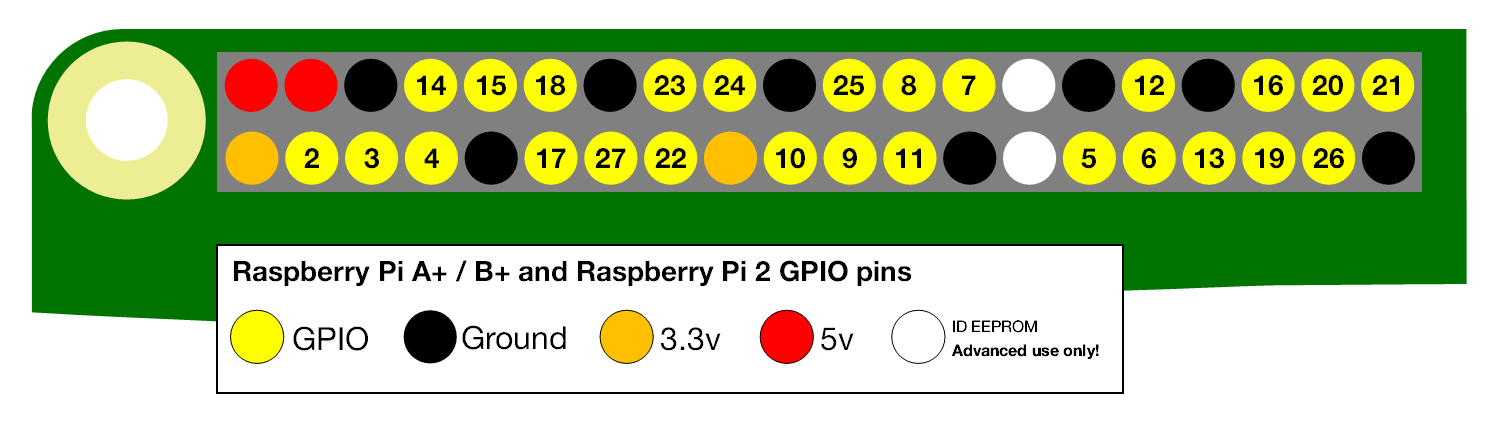
\includegraphics[width=\textwidth]{Bilder/Kapitel2/gpio_pins_pi2.png}
	\caption[Schema GPIO Pins]{Schematische Darstellung der GPIO Pins. Entnommen aus der Raspberry Pi Dokumentation\cite{GPIOMode77:online}.}
	\label{fig:Kapitel2/gpio_pins_pi2.png}
\end{figure}
\noindent
An den vorhandenen 3.3V und 5V Anschlüsse können Sensoren betrieben werden. Dennoch sind nicht alle Sensoren verwendbar. Der Raspberry Pi verfügt nur über die Möglichkeit digitale Signale an den \ac{GPIO} Pins zu verarbeiten. Es werden jedoch neben digitalen auch analoge Sensoren benötigt. Diese können nicht direkt an die Pins angeschlossen werden, aber das Problem wird mit einem \ac{A/D-Wandler} gelöst. \\
Die Erweiterungsplatine RPi-Explorer 700 von Joy-IT \cite{joyitrpi87:online} beinhaltet einen \ac{A/D-Wandler} an dem Analoge Pins angeschlossen werden können. Durch die Erweiterung ist es möglich bis zu vier analoge Sensoren an einem Sensorknoten betrieben werden. \\
Die \ac{GPIO} Schnittstelle unterstützt nur eine maximale Versorgungsspannung von 3.3V, was für die Sensoren ausreichend ist. Durch die Kompatibilität zum Arduino und dem Raspberry Pi können die Sensoren sowohl mit 5V als auch mit 3.3V betrieben werden.
Folgende Sensoren von Allnet\cite{111861pd90:online} werden  im \fullref{Verdrahtung_der_Sensoren} verwendet:
\begin{description}
\item[Temperatur und Luftfeuchtigkeitssensor] \hfill \\
	Der Sensor, KY-015, vom Typ DHT11 kann Temperaturen von 0 bis 50$^\circ$C mit einer Messungenauigkeit von $\pm$ 2$^\circ$C. Die Luftfeuchtigkeit kann im Bereich von 20 bis 95\% ($\pm$ 5\%) gemessen werden. Hierbei handelt es sich um einen digitalen Sensor.  
\item[Flammensensor]\hfill \\
	Der KY-026 besteht aus einer Fotodiode und einem \ac{Poti}. Die Fotodiode kann Wellenlängen im Bereich von etwa 720 - 1100 nm detektieren. Die Diode hat einen Erfassungswinkel von etwa 60$^\circ$. Der \ac{Poti} wird zur Empfindlichkeitseinstellung genutzt, somit kann eine Reichweite von etwa  ein bis sieben Metern abgedeckt werden. Der Sensor besitzt einen "'Digital Out"'-Pin, der high active geschalten wird. Sobald eine Flamme erkannt wird, liegt eine logische 1 auf dem Pin. Der "'Analog Out"'-Pin liefert ein analoges Signal, an welchem bei einer gemessenen Flamme eine niedrige Spannung anliegt.
\item[Lichtschranke]\hfill \\
	Das KY-010 Modul ist eine Lichtschranke, die beim Unterbrechen eine logische 1 an dem digitalen Ausgangspin liefert.
\item[Mikrofon]\hfill \\
	Das Mikrofon, KY-038, hat den gleichen Aufbau wie der Flammensonser. Im Gegensatz zum Flammensensor wird hierbei ein Mikrofonmodul, statt einer Fotodiode genutzt. Die Signale am Digital Out und Analog Out haben die gleiche Funktionalität wie beim Flammensensor. Dieses Modul dient hauptsächlich zur Detektion von kurzen aber lauten Tönen. Ein Anwendungsbeispiel hierfür ist eine Alarmfunktion. Beispielsweise kann das Zerbrechen eines Fensters festgestellt werden.
\item[Lichtsensor]\hfill \\
	Der Lichtsensor KY-018, bestehend aus einem Fotowiderstand, hat bei Dunkelheit einen Widerstand $>$20M$\Omega$ und bei Helligkeit $<$ 80$\Omega$. Damit kann bestimmt werden, ob in einem Zimmer das Licht brennt. Der Lichtsensor liefert ein analoges Signal.
\item[Schocksensor]\hfill \\
	Der Erschütterungssensor liefert eine logische 1 an dem Ausgangspin, falls eine Erschütterung festgestellt wurde. Das dient exemplarisch zur Umsetzung einer Schritterkennung am Boden.
\end{description}

%Harm
\section{WLAN}
\subsection{Standard}
Die \ac{IEEE} hat 1997 den Standard 802.11 veröffentlicht. Der Standard sieht vor, dass im 2,4 GHz-Band eine Datenrate von 1-2 Mbit/s gewährleistet ist. 1999 ist der Standard durch 802.11a und 802.11b erweitert worden. 802.11a sieht vor, dass im 5 GHz-Band eine Datenrate von 54 Mbit/s möglich ist. 802.11b funkt im 2,4 GHz-Band und bietet eine Datenrate von 11 Mbit/s. 2003 ist 802.11g veröffentlicht worden welcher auch im 2,4 GHz-Band Datenraten von 54 Mbit/s ermöglicht. Im September 2009 ist der Standard 802.11n veröffentlicht worden. Dieser Standard ermöglicht Datenraten von bis zu 150 Mbit/s. Wird 4x4-Mimo verwendet sind theoretisch sogar bis zu 600 Mbit/s möglich. Als Frequenzband sind sowohl das 2,4 GHz-Band als auch das 5 GHz-Band erlaubt.
 

\subsection{Verschlüsselung}

Da WLAN die Luft als Übertragungsmedium verwendet und jeder darauf zugreifen kann, verdient die Verschlüsselung des Datenverkehrs besondere Aufmerksamkeit. Die Verschlüsselung verhindert, dass dritte die Kommunikation des Endgeräts mit dem Access-Point mitlesen können. Verschlüsselung hat allerdings das Problem, dass beide Geräte ein Geheimnis teilen müssen. Dieses Geheimnis wird Schlüssel genannt. Es gibt aktuell drei Verschlüsselungsverfahren, die verwendet werden können. \ac{WEP} und \ac{WPA} sind aber bereits geknackt und somit nicht mehr sicher.

\subsubsection{\ac{WEP}}
Bei der Standardisierung des Standards 802.11b, 802.11g und 802.11a wurde \ac{WEP} integriert. \ac{WEP} basiert auf einem Stream Ciphering-Algorithmus, bei dem die Daten mit einer Ciphersquenz verschlüsselt werden. Die Sequenz wird mit einem \ac{IV} und einem Schlüssel berechnet. Der \ac{IV} ändert sich für jedes Frame und erzeugt somit wechselnde Ciphering Keys. Der daraus berechnete Schlüssel wird mit den Daten der Nachricht verodert. (vgl. \cite{SWB-430171331})


\begin{figure} [htb]
\begin{centering}
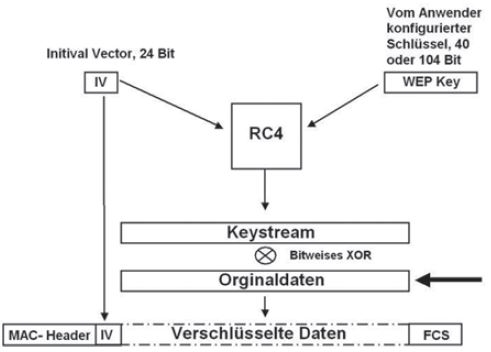
\includegraphics{Bilder/wep_funktionsweise.jpg}
\caption[WEP-Verschlüsselung]{WEP-Verschlüsselung \cite{SWB-430171331}}
\label{wep_funktionsweise}
\end{centering}
\end{figure}

Problematisch an diesem Verfahren ist, dass der Schlüssel bei jedem Teilnehmer eingetragen werden muss und somit nicht Geheim gehalten werden kann. Schwerwiegender ist allerdings, dass jedes verschlüsselte Frame am Anfang die gleiche Bytefolge des \ac{LLC}-Headers beinhaltet. Bestimmte \acp{IV} werden im Klartext übertragen wodurch ein Angreifer nach 5-6 Millionen Paketen den Schlüssel berechnen kann. Mittlerweile sind auch Anwendungen verfügbar, die selbst Datenpakete erzeugen und so in sehr kurzer Zeit, den Schlüssel berechnen können.(vgl. \cite{SWB-430171331})
%TODO: Kann bei Seitenbedarf noch ausgebaut werden

\subsubsection{\ac{WPA}} 
%TODO: Schluessel in PPE-Schluessel muss geändert werden. Mal mit Alex sprechen warum das ü nicht gefressen wird
Da \ac{WEP} die beschriebenen Schwächen hat ist 802.11i von der \ac{IEEE} entwickelt worden. Da \ac{WPA2} aber \ac{CCMP} voraussetzt, was mehr Leistung benötigt, wurde durch die Industrie \ac{WPA} entwickelt. \ac{WPA} funktioniert auch auf schwächerer Hardware. Als Verschlüsselungsmethode wird \ac{TKIP} und Optional \ac{CCMP} verwendet. Beschrieben wird hier die Funktionsweise mit \ac{TKIP}. \\
\ac{TKIP} verwendet wie \ac{WEP} den RC4-Algorithmus zur Verschlüsselung der Daten aber der Umgang mit Daten und Schlüsseln ist komplexer. \\
Nach \textsc{Klaus Schmeh} \cite{SWB-378541420} ist die Grundlage von \ac{TKIP} der \ac{PMK}, der beiden Seiten bekannt sein muss. Er hat eine Länge von 256 Bit und wird nur zur Ableitung anderer Schlüssel verwendet. Aus einem \ac{IV}, der MAC-Adresse und dem Daten-Schlüssel wird ein \ac{PPE}-Schlüssel gebildet. Der \ac{PPE}-Schlüssel ist 128 Bit lang und wird für jedes Datenpaket neu generiert.
Der \ac{IV} teilt sich in zwei Teile von denen der erste 16 Bit und der zweite 32 Bit lang ist. Dies ergibt eine Länge von 48 Bit was bereits mehr ist als der 24 Bit \ac{IV} von WEP. Der erste Teil erhöht sich von Paket zu Paket um 1.\\
Wie aus der Grafik (\nameref{wpa_funktionsweise}) hervorgeht werden der MICHAEL-Schlüssel und die unverschlüsselten Daten an die schlüsselabhängige Hashfunktion MICHAEL übergeben, die einen Hashwert berechnet. Die Daten und der Hashwert werden zusammengefügt und es wird mit CRC ein zweiter Hashwert generiert. Verschlüsselt werden die Daten mit den beiden Hashwerten nun mit dem RC4-Verfahren und dem jeweils gültigen \ac{PPE}-Schlüssel. (vgl. \cite{SWB-378541420})

\begin{figure} [htb]
\begin{centering}
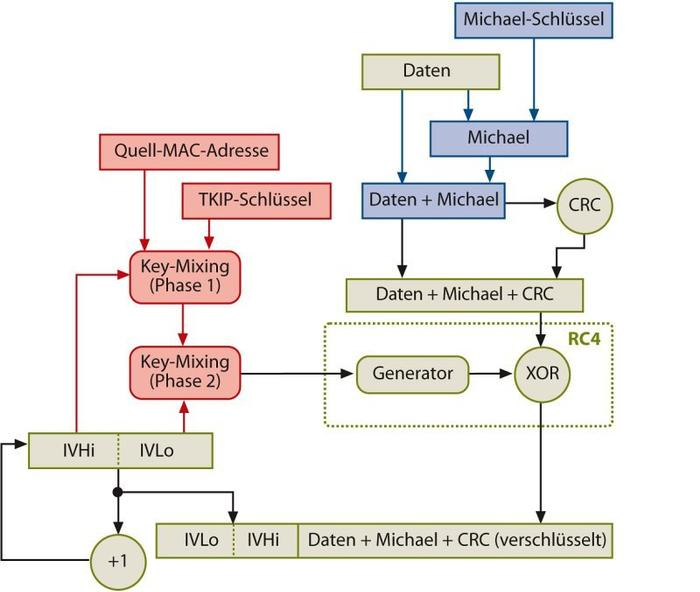
\includegraphics[scale=0.6]{Bilder/wpa_funktionsweise.jpg}
\caption[WPA-Verschlüsselung]{WPA-Verschlüsselung \cite{Heise-WLAN}}
\label{wpa_funktionsweise}
\end{centering}
\end{figure}

\subsubsection{\ac{WPA2}}
\ac{WPA2} und \ac{WPA} sind nahezu identisch. \ac{CCMP} ersetzt \ac{TKIP} und die Hashfunktion MICHAEL. \ac{CCMP} basiert auf dem \ac{AES}-Verschlüsselungsstandard. (vgl. \cite{WPA2}
%TODO: Falls jemand eine Idee hat wie man das noch ausschmücken kann... her damit!!!!
\newpage

\chapter{Planung}
Bevor mit der Umsetzung begonnen wird, muss geklärt werden, welche Schritte notwendig sind und in welcher Reihenfolge sie sinnvoll sind. Die Planung schafft die Grundlage auf der die spätere Umsetzung aufsetzt um eine reibungslosere Entwicklung zu ermöglichen.

%Harm
\section{Zeitplanung}\label{Zeitplanung}
Zuerst muss sich über das Themengebiet informiert werden. Danach erfolgt der
Entwurf eines Konzepts mit daran anschließender Technologieauswahl. Nachdem die
Technologieauswahl getroffen ist wird die notwendige Hardware beschafft und
parallel dazu mit der Aufteilung der Aufgaben in Arbeitspakete begonnen. Im
nächsten Schritt werden die Arbeitspakete in logischer Abfolge abgearbeitet und
das Konzept so schrittweise umgesetzt.\\
Die Zeitplanung ist Semesterbedingt in zwei große Blöcke unterteilt.\\
Im ersten Semester werden folgende Punkte umgesetzt:

\begin{enumerate}
	\item Informationsphase
	\item Entwicklung eines Konzeptes
	\item Technologieauswahl
	\item Beschaffung von notwendiger Hard- und Software
	\item Aufteilung der Aufgaben in Arbeitspakete
	\item Erstellen der Zeitplanung
\end{enumerate}

Im zweiten Semester werden folgende Punkte umgesetzt:

\begin{enumerate}
	\item Abarbeitung der Arbeitspakete
	\item Erstellung der Dokumentation
\end{enumerate}
%Jan
\subsection*{GANTT-Diagramm}
Die geannten Punkte des Kapitels \nameref{Zeitplanung} müssen zeitlich strukturiert in einem GANTT-Diagramm festgehalten werden.
Die folgenden GANTT-Diagramme wurden im Rahmen der Zeitplanung erstellt:
\begin{landscape}
	\begin{figure}[h]
		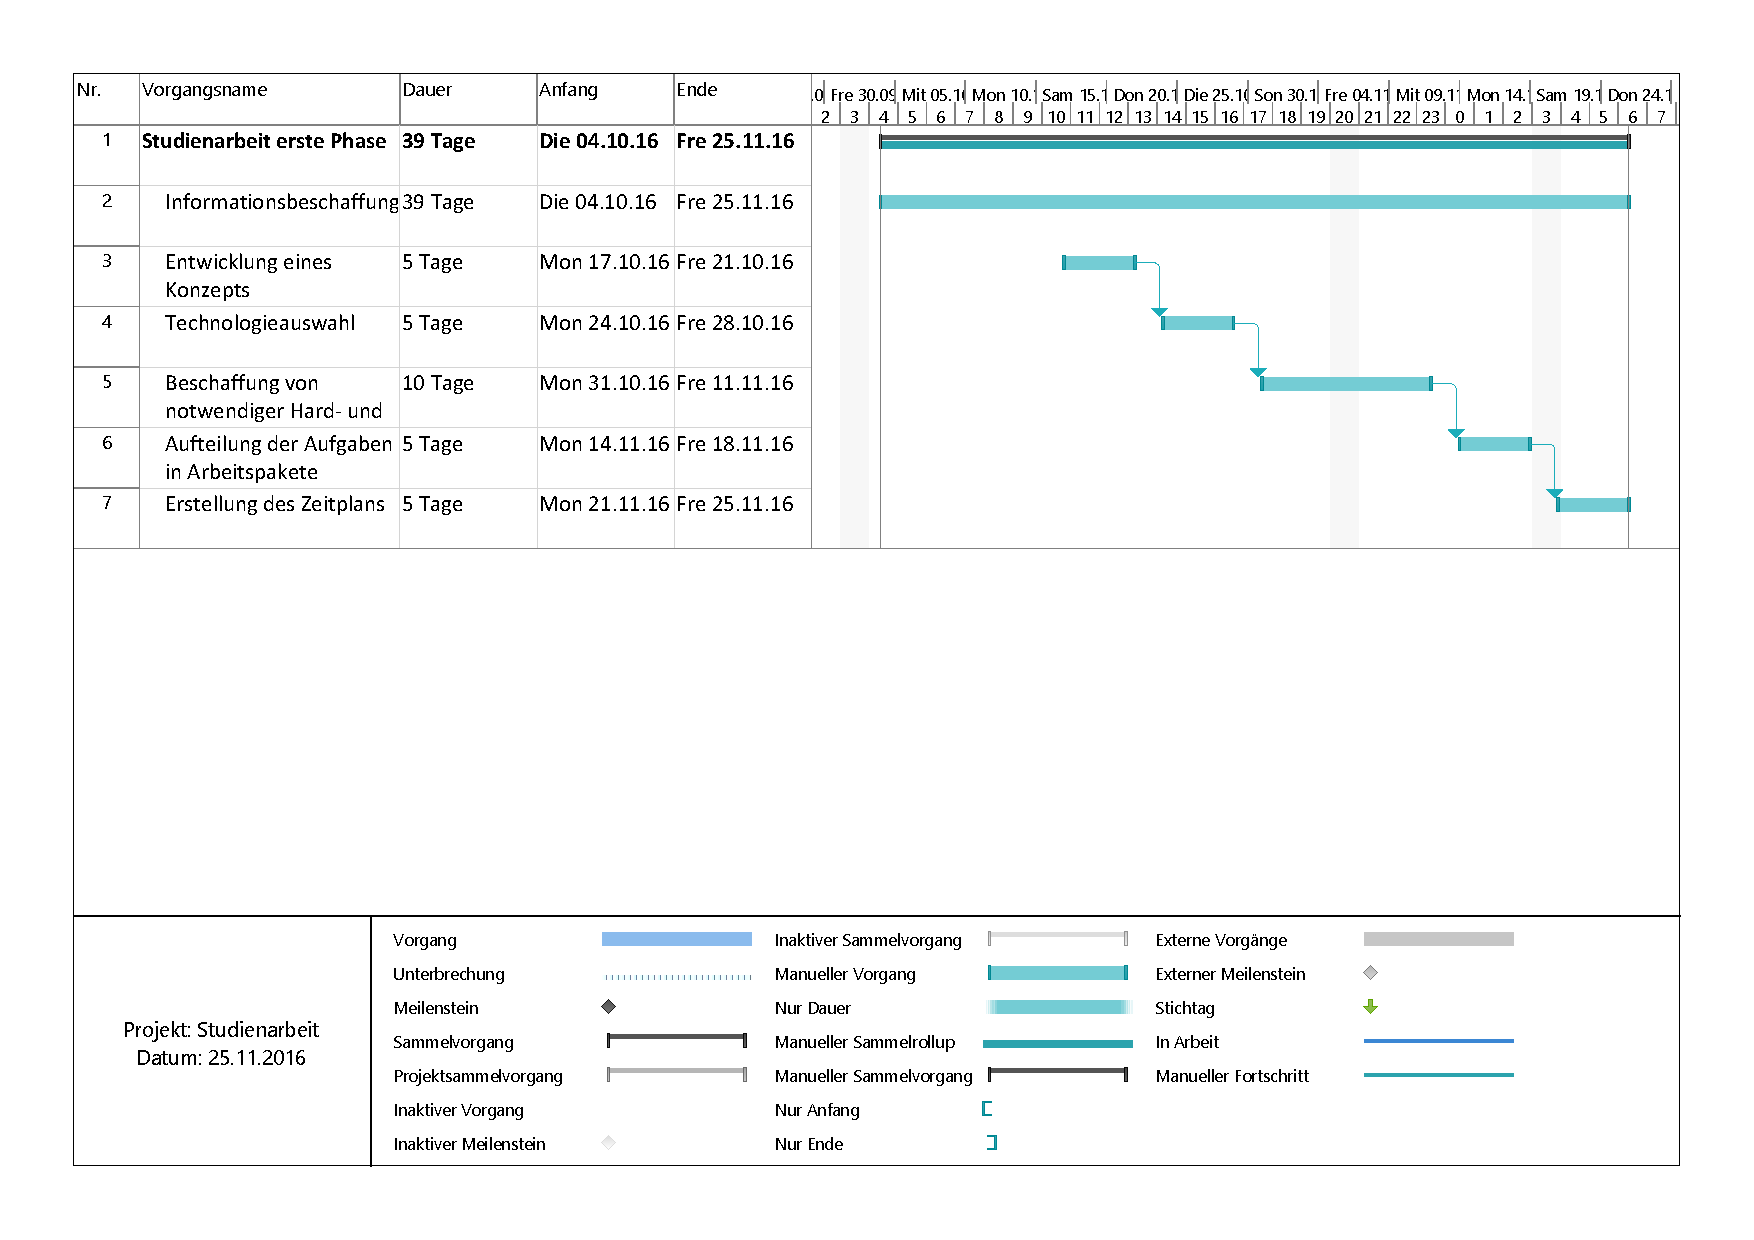
\includegraphics[width=\linewidth, height=.9\textheight]{Bilder/GANTT/Studienarbeit_erste_Phase.pdf}
		\caption[CaptionTitle]{TEXT}
		\label{fig:}
	\end{figure}
\end{landscape}



\section{Netzwerkplanung}
Eine zentrale Funktionalität ist die Datenübertragung weshalb das Netzwerk eine besonders kritische Komponente ist. Das Netzwerk ist so auch eines der ersten Komponenten, die funktionieren muss, damit beim späteren Entwickeln auf eine funktionierende Infrastruktur zurückgegriffen werden kann.
%Harm
\subsection{Netzwerkplan}
%TODO: Einleitungssatz
Die Sensoren sind an den Sensorknoten angeschlossen. Die Daten werden per WLAN
an die Zentraleinheit gesendet. Dort werden die Daten in die Datenbank
geschrieben.\\
Der Webserver greift auf die Datenbank zu und stellt die Daten auf einer Website
übersichtlich dar. (\nameref{Darstellung_Umgebung})
%TODO: Feinschliff Netzplan
\begin{figure} [htb]
\begin{centering}
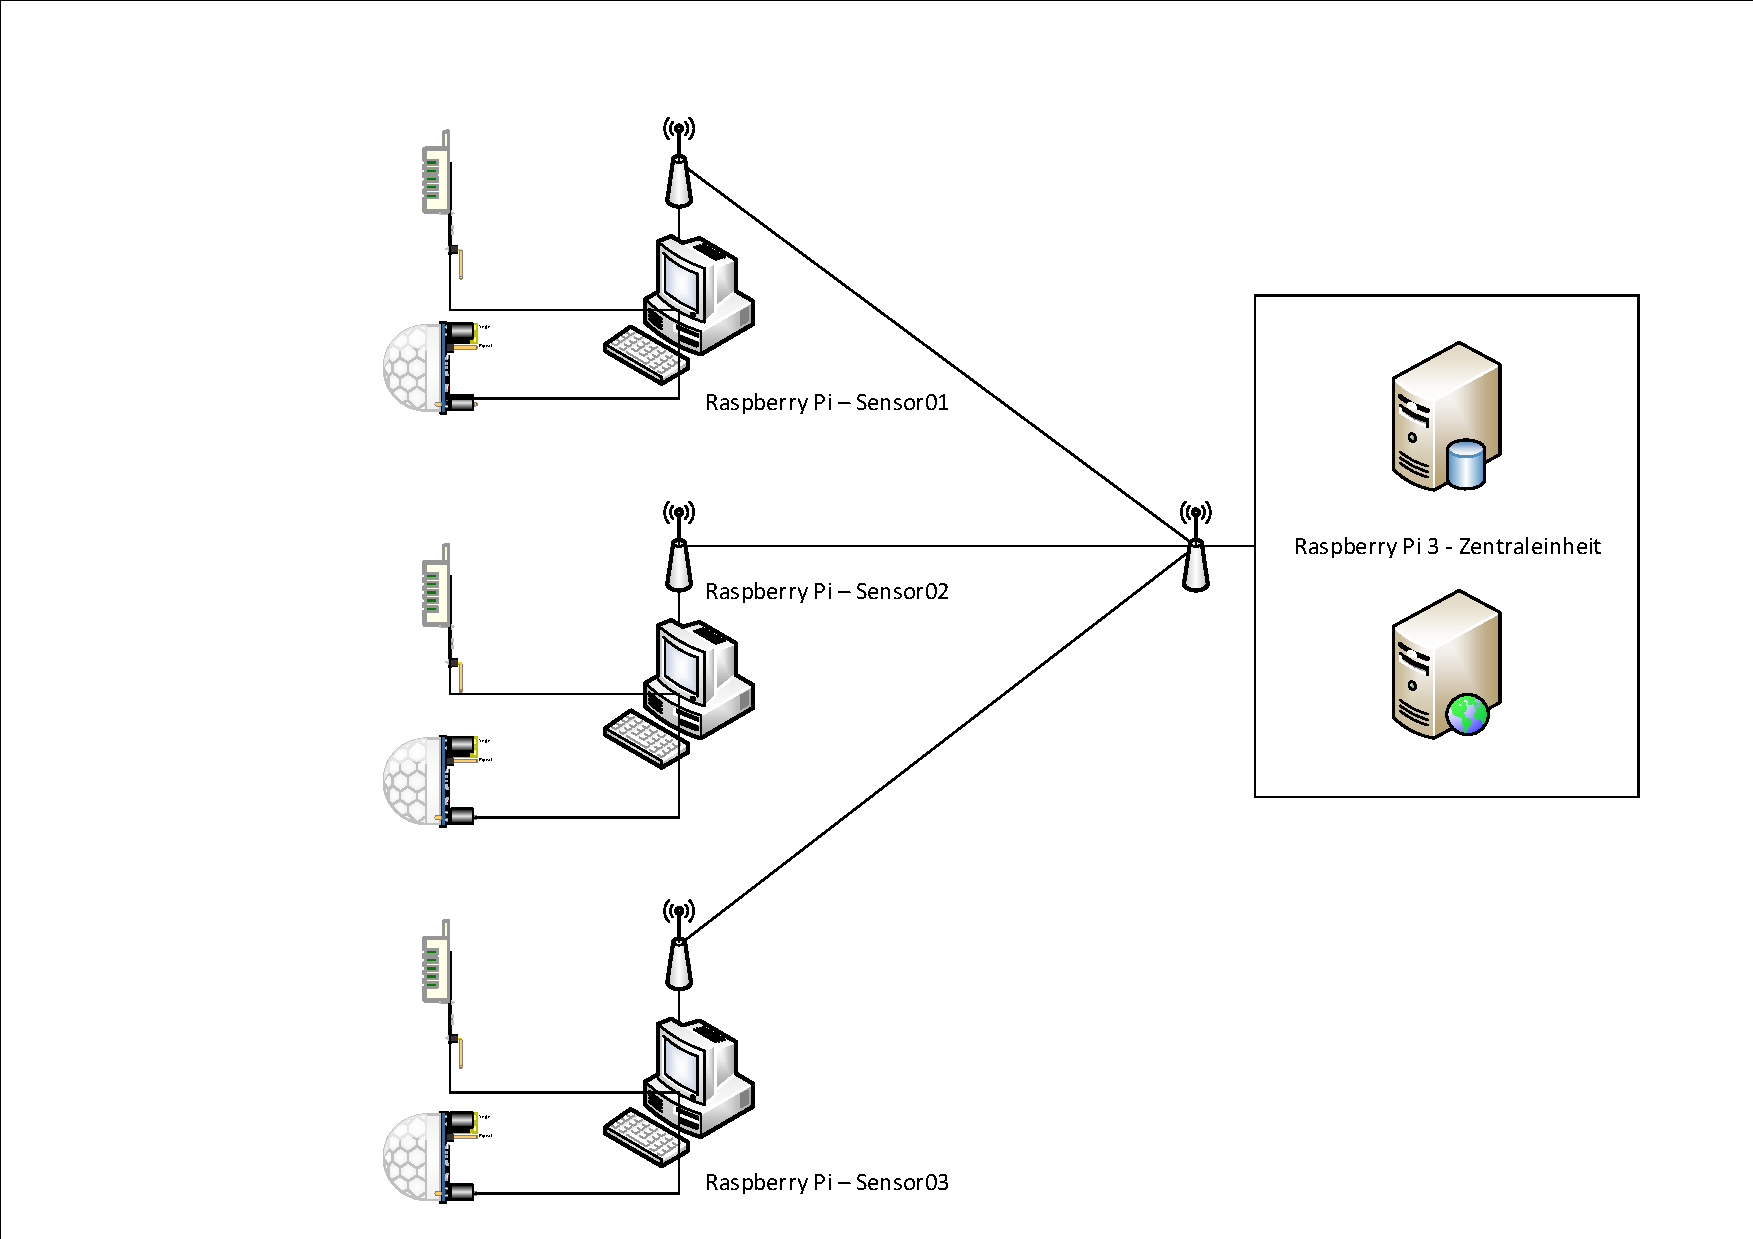
\includegraphics[scale=0.4]{Bilder/Netzplan.pdf}
\caption[Schematische Darstellung der geplanten Umgebung]{Schematische
Darstellung der geplanten Umgebung}
\label{Darstellung_Umgebung}
\end{centering}
\end{figure} 

%Harm
\subsection{Kommunikation}
%Bsp
Für die Kommunikation der einzelnen Komponenten ist ein DHCP-Server, der über das WLan eine Verbindung zwischen der Zentraleinheit und der Sensorknoten herstellt.
%TODO: Schnittstelle erwähnen

%Alex
\section{Sensorknoten}
%TODO: Erwähnen, dass mehrere Sensorknoten geben kann
Ein Raspberry Pi, an dem die Messdaten der Sensoren gesammelt werden, wird als Sensorknoten bezeichnet. An diesen können bis zu sieben Sensoren, die im Kapitel \nameref{Sensoren_Planung} beschrieben sind, angeschlossen werden. Neben dem Messen muss der Sensorknoten die Messdaten an die Zentraleinheit weiterleiten, welche die Daten auswertet. Bevor der Sensorknoten implementiert werden kann, muss eine Auswahl der Programmiersprache getroffen werden.
%Jan
\subsection{Python vs. Java}
Für das Projekt ist die richtige Programmiersprache essenziell. Die Sprache muss nicht nur die Daten der Sensoren auslesen, sondern diese auch in Pakete packen und an die Zentraleinheit weitergeben. Die Weitergabe der Datenpakete soll über eine Schnittstelle erfolgen, die von der ausgewählten Sprache erstellt werden kann. Hierzu werden zwei Programmiersprachen verglichen, \nameref{Java} und \nameref{Python}. Folgende Tabelle vergleicht die Funktionaliäten der Sprachen, die für das Projekt notwendig sind:\hfill

\begin{table}[h]
	\centering
	\caption{Python vs. Java}
	\label{tab:phytionvsjava}
	\begin{tabular}{l|l|l}
	\textbf{Funktionalität} & \textbf{Java} &\textbf{Python}   \\
	\hline
	 Speicherverbrauch & hoch & niedrig \\\hline
	Komplexität  & hoch & niedrig\\\hline
	Geschwindigkeit  & hoch & hoch \\\hline
	Bibliotheken für die Sensoren & nicht vorhanden & vorhanden \\\hline
	Schnittstelle für die Datenübertragung & vorhanden & vorhanden
	\end{tabular}
\end{table}
\noindent Da die Raspberry Pi's für schnelle kleine hardwarenahe Projekte ausgelegt sind, fiel die Entscheidung auf die Sprache Python. Java nur bedingt hardwarenah ist und die Speicherkapazität der Raspberry Pi's begrenzt ist. Ein weiterer Vorteil von Python, sind die bereits vorhandenen Bibliotheken und die kurze Einarbeitungszeit. Die kürzere Einabreitungs- und Umsetzungszeit, kommt der engmaschigen \nameref{Zeitplanung} zu gute. %TODO: Verweis auf den Zeitplan

%Alex
\subsection{Auslesen der Sensoren}
%TODO: Priorisierung der Sensoren
%TODO: Allgemeine Messdatenformat
%Jan
\section{Zentraleinheit}
%Jan
\subsection{Datenbank}
%Harm
\subsection{Website}

Auf der Website soll sich ein Benutzer einloggen oder registrieren können.
Nach dem Login soll der Benutzer zu einer Übersicht weitergeleitet werden, auf der alle Sensorknoten in
Tabellenform abgebildet sind mit den aktuell gemessenen Werten. \\
Auf einer Statistik-Seite soll ein Verlauf über mehrere Tage zu einem Sensor sichtbar sein.\\
Eine Webcam-Seite soll dazu dienen, auf eine angeschlossene Webcam zuzugreifen.\\
Ein Impressum soll eine kurze Information anzeigen, wer dieses Projekt umgesetzt hat.\\
Auf einer Logout-Seite soll der Benutzer die Meldung sehen, dass er ausgeloggt ist und eine Möglichkeit angeboten bekommen um zurück zur Login-Seite zu gelangen.
(\nameref{Darstellung_Website_einfach})

\begin{figure} [htb]
\begin{centering}
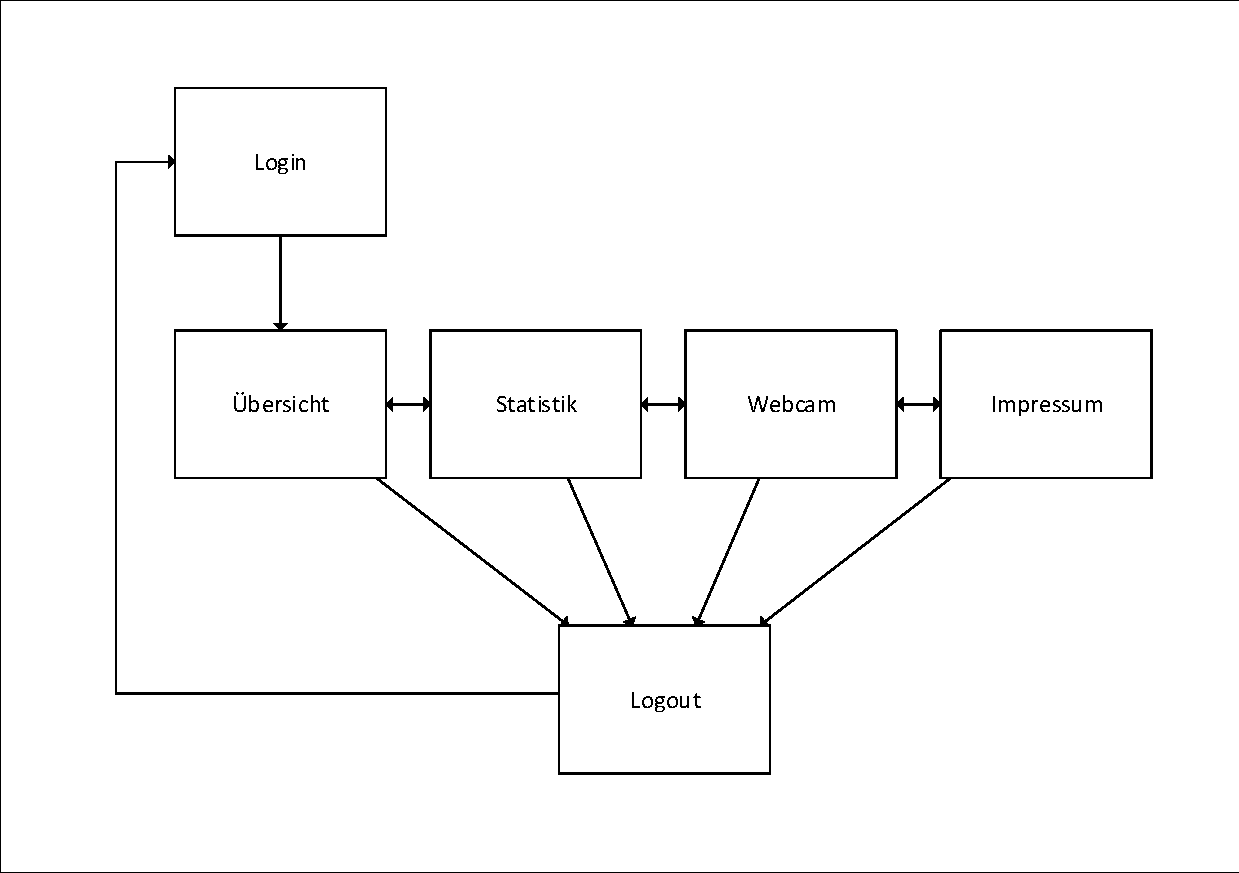
\includegraphics[scale=0.8]{Bilder/struktur_website_einfach.pdf}
\caption[Schematische Darstellung der geplanten Website]{Schematische
Darstellung der geplanten Website}
\label{Darstellung_Website_einfach}
\end{centering}
\end{figure}

%Alle
\section{Planungsresultat}
%TODO: Wortwahl: kein "werden" sondern "sollen"
Die Sensoren werden kontinuierlich abgefragt und senden die gemessenen Werte an
die Datenbank auf der Zentraleinheit. Dort werden die Daten entsprechend dem
meldenden Sensorknoten abgespeichert. Die Website greift auf die Datenbank zu
und lädt die Daten in eine tabellarische Darstellung, die der Benutzer dann
sieht. Durch einen Zeitstempel ist es möglich bei Daten der Temperatursensoren
und der Feuchtigkeitssensoren einen Verlauf darzustellen.

\newpage

\chapter{Umsetzung}

Die Sensoren werden an einen Raspberry Pi angeschlossen und melden die
gemessenen Werte an einen zentralen Raspberry Pi. Der zentrale Raspberry Pi legt
die gemeldeten Daten in einer Datenbank ab. Eine Website greift auf die
Datenbank zu und stellt die Daten dar.\\
Die Kommunikation wird über ein eigenes WLAN-Netz abgewickelt das von der
Zentraleinheit aufgespannt wird. IP-Adressen werden von einem DHCP-Server, der
auf der Zentraleinheit installiert ist vergeben.\\
Die Website wird durch einen Apache-Webserver auf der Zentraleinheit
bereitgestellt.

\section{Netzwerkkonfiguration}


\subsection{WLAN}

Es wird ein Funknetz auf Basis des 802.11n Standards verwendet. Als Name wurde
Pinet festgelegt, der von allen gesehen werden kann. In der Tabelle
(\nameref{tab:WLAN-Konfiguration}) sind die einzelnen Optionen
aufgeführt und erläutert.


\begin{table}
\caption{WLan-Konfigurationsdetails}
\label{tab:WLAN-Konfiguration}
\begin{tabular}{p{0.5\textwidth} p{0.45\textwidth}}
Befehl & Erklärung \\
interface=wlan0 & Das Interface auf dem das Funknetz ausgestrahlt wird \\
ssid=Pinet & Der name des Funknetzes \\
country\_code=DE & Über die Festlegung der Region wird sichergestellt, dass das
Funknetz die spezifischen Grenzwerte für Kanäle oder Sendestärke einhält \\
hw\_mode=g & legt fest, dass das Funknetz im 2,4 GHz-Band ausgestrahlt wird \\
channel=6 & Der Funkkanal 6 wird verwendet \\
macaddr\_acl=0 & MAC-Adressenfilterung ist deaktiviert \\
auth\_algs=1 & Legt fest, dass als Verschlüsselung WPA verwendet wird \\
ignore\_broadcast\_ssid=0 & Die SSID wird ausgestrahlt und nicht versteckt. \\
wpa=2 & Legt die WPA-Version fest auf WPA2 \\
wpa\_passphrase=IrgendeinbloedesPasswort & Legt den Pre-Shared-Key fest \\
wpa\_key\_mgmt=WPA-PSK & Legt fest, dass ein Pre-Shared-Key verwendet wird \\
wpa\_pairwise=CCMP & Legt fest, dass nur der AES-Verschlüsselungsalgorithmus
verwendet wird \\
wpa\_group\_rekey=86400 & Legt fest, dass alle 86400 Sekunden ein neuer
Schlüssel verwendet werden muss \\
ieee80211n=1 & Aktiviert den n-Standard \\
wme\_enabled=1 & Aktiviert Quality-of-Service - Voraussetzung für die Verwendung
des n-Standards \\
 \end{tabular}
\end{table}

\subsection{Verschlüsselung}

Wie aus der Tabelle WLAN-Konfigurationsdetails (\nameref{tab:WLAN-Konfiguration}) hervorgeht ist das WLAN mit WPA2 verschlüsselt. WPA2 gilt aktuell als sicher, was nicht für die Alternativen WEP oder WPA gilt. Zur Authentifizierung wird ein Pre-Shared-Key (PSK) verwendet. Als Verschlüsselungsprotokoll wird CCMP verwendet. 

\subsection{DHCP}

Als DHCP-Server wird der ISC-DHCP-Server verwendet.\\
Die IP-Adressen werden nur über das wlan0-Interface der Zentraleinheit vergeben.
Als Netz wurde das Private Netz 192.168.178.0 /24 verwendet. In diesem Netz hat
Die Zentraleinheit als DHCP-Server die Adresse 192.168.178.1 /24. Diese Adresse
ist Statisch eingetragen. Alle anderen Geräte erhalten dynamische IP-Adressen
aus dem Bereich 192.168.178.10 - 192.168.178.250. Die Lease-Time wurde auf
604800 sekunden festgelegt. Dies entspricht 7 Tagen. Da nur wenige Geräte im
Netz verfügbar sind und auch keine häufigen Änderungen erwartet werden wird dies
als ausreichend angesehen.

\begin{verbatim}
/etc/dhcp/dhcpd.conf

#Rogue-DHCP-Server nicht erlauben (Doppelter DHCP-Server)
authoritative;

#Definition des Subnetzes
subnet 192.168.178.0 netmask 255.255.255.0
{
        #Angabe der DHCP-Range
        range 192.168.178.10 192.168.178.250;

        #Angabe der Lease-Times 7 Tage in sekunden
        default-lease-time 604800;
        max-lease-time 604800;

        #Begrenzung auf das WLAN-Interface
        interface wlan0;
}

\end{verbatim}

\subsection{Mesh}
\section{Sensorknoten} %Allgemein Vorinstalation!
%TODO: Notwendige Librarys
Python bietet mit Hilfe der Adafruit\cite{Adafruit60:online} Bibliotheken eine Schnittstelle zu den Sensoren. Die Adafruitbibliothek kann mithilfe des pythoneigenen Packetmanager installiert werden.
\begin{verbatim}
pip install adafruit_python_dht
\end{verbatim}
Dieses Packet wird zum Ansteuern des DHT-11 Sensors benötigt.
\subsection{Verdrahtung der Sensoren}

\subsection{Implementierung der Sensoren}
\subsection{Konfiguraton \& Testen der Sensoren}
\subsection{Priorisierung der Sensoren}
\subsection{Übertragung der Sensordaten}

\section{Zentraleinheit}%Allgemein Vorinstalation!
\subsection{Empfagen der Sensordaten}
\subsection{Befüllen der Datenbank}
\subsection{Problematik Zeitsynchronisierung}
 
\section{Website}

\subsection{Login}

Der Login, die Registrierung und der Logout ist nach der Anleitung von
wikiHow erstellt und entsprechend angepasst worden. (\cite{PHP-Login})
\\
Der Login besteht aus mehreren Dateien, deren Funktion in der Tabelle
(\nameref{tab:Login-Dateien}) aufgezählt ist.

\begin{table}
\caption{PHP-Login-Dateien und Funktion}
\label{tab:Login-Dateien}
\begin{tabular}{p{0.5\textwidth} p{0.45\textwidth}}
Datei & Erklärung \\
Login.php & Die Loginseite - Gleichzeitig auch die Startseite bei Aufruf der
Server-IP\\
Register.php & Die Registrierungsseite \\
Register\_success.php & Die Seite, die nach einer erfolgreichen Registrierung
angezeigt wird \\
Logout.php & Die Seite, die nach einem erfolgreichen Logout angezeigt wird \\
psl\_config.php & Festlegung von Variablen, die mehrfach verwendet werden \\
db-connect.php & Datenbank-Connector \\
functions.php & Relevante Funktionen, die benötigt werden \\
process\_login.php & Code der die Logindaten der Loginseite überprüft und danach
weiterleitet \\
register\_inc & Code der abläuft wenn sich ein User neu registriert \\
forms.js & Javascriptdatei, für das Hashen und überprüfen der Passwörter \\
sha512.js & Hashfunktion \\
style.css & CSS-Datei für zentrale Designeinstellungen \\
 \end{tabular}
\end{table}

In der Datei functions.php sind zentrale Funktionen gesammelt, die nachfolgend
beschrieben werden:

\subsubsection{sec\_session\_start}
Diese Funktion vergibt eine Session-ID und legt fest, dass Cookies verwendet werden.

\subsubsection{login}
Diese Funktion steuert alle notwendigen Abläufe den Login betreffend.\\
Aufgerufen wird die Funktion mit den Parametern Username, Passwort und der Datenbankverbindung. Die Parameter Username und Passwort werden aus POST-Werten der Loginseite übergeben während die Datenbankverbindung in der Datei db-connect.php definiert ist. Durch ein Prepared-Statement werden die Werte mit den eingetragenen Werten der Datenbank verglichen. Existiert der Benutzer, wird zuerst überprüft ob der User momentan gesperrt ist durch die Funktion 'checkbrute'. Ist dies nicht der Fall wird das Passwort überprüft und der Anwender wird gegebenenfalls auf die Seite 'Übersicht' weitergeleitet. Ist das Passwort nicht korrekt wird der fehlgeschlagene Loginversuch in der Datenbank vermerkt.

\subsubsection{checkbrute}

\subsubsection{login\_check}
Diese Funktion prüft ob ein Anwender eingeloggt ist und setzt den entsprechenden
Parameter, der dann entscheidet was der Anwender auf der Website sieht.

\subsubsection{esc\_url}


\subsection{Übersicht}

\subsection{Statistik}

\subsection{Webcam}

\subsection{Impressum}

\section{Refactoring}
\section{Systemtest}

\newpage

\chapter{Fazit}

\section{Problemstellungen}
Bsp: Mesh

\section{Ausblick}

\section{Persönliches Fazit}
\newpage

%%%%%%%%%%%%%%%%%%%%%%%%%%%%%%%%%%%%%% URL wegen Sonderzeichen Vordefinieren %%%%%%%%%%%%%%%%%%%%%%%%%%%%%%%%%%%%%%%%%%%%%%%%%%%%%%%%%%%%%%%%%%%%%%%

%\urldef{\newUrl}\url{http://www.htl-hl.ac.at/el/projekte/2011/DA_Spielekonsole/Sonstiges/GanttProject%20Tutorial.pdf}

%%%%%%%%%%%%%%%%%%%%%%%%%%%%%%%%%% Literaturverzeichnis %%%%%%%%%%%%%%%%%%%%%%%%%%%%%%%%%%%%%%%%%%%%%%%%%%%%%%%%%%%%%%%%%%%%%%%%%%%%%%%%%%%%%%%%%%

\addcontentsline{toc}{chapter}{Literaturverzeichnis}
%\bibliographystyle{gerabbrv}					% Zitierformat (deutsch für Großschreibung)
% [Häufigkeit] im Text
%\bibliography{Literaturverzeichnis}		% Pfad des Literaturverzeichnisses.bib

\printbibliography

\newpage
\thispagestyle{plain}
\section*{Anhang}

							% Anhang Einbinden

\end{document}